%%% Fiktivní kapitola s ukázkami sazby

\chapter{Technologie}

Kapitola technologie se zabývá využitými technologiemi a jakým způsobem byly vybrány. Jednotlivé technologie jsou představeny pro porozumění následující kapitole návrh, který byl proveden s ohledem na vybrané technologie.

Pro výběr technologií byla stanovena následující kritéria:

\begin{itemize}
	\item podpora platforem iOS a Android,
	\item rychlost vývoje,
	\item velikost komunity a aktuálnost dokumentace,
	\item programovací jazyk,
	\item jednoduchost vytváření UI,
	\item dostupnost potřebných komponent pro aplikaci.
\end{itemize}

Jednotlivá kritéria jsou rozebrána níže.

% vlastní oddělení

\section{Kritéria výběru}

\subsection{Podpora více platforem}

Podpora platforem iOS a Android je kritickým požadavkem aplikace vycházející z analýzy požadavků. Technologie musí podporovat, ideálně platformně nezávisle abstrahovat, přístup k zdrojům souborového systému, přístup k vzdáleným zdrojům pomocí protokolu HTTP, umožnit vytvářet mapové aplikace, bezpečně uložit uživatelské přihlašovací údaje. Technologie by neměla vyžadovat platformně závislý nativní kód.

\subsection{Rychlost vývoje}

Rychlost vývoje je obtížně kvantifikovatelnou veličinou. Do rychlosti vývoje lze zahrnout mnoho aspektů a záleží, z jakého pohledu se na problematiku pohlíží. Z pohledu řízení projektu se může např. jednat o počet dostupných vývojářů a doba adaptace na technologii. Z pohledu programátora se může jednat o kvalitu a dostupnost vývojových nástrojů, dostupnost knihoven, přehlednosti kódu, dostupné funkce programovacího jazyka technologie. Z pohledu údržby se může jednat o očekávanou životnost technologie nebo dostupnosti testovacích nástrojů. Kombinací těchto aspektů může vzniknout více či méně subjektivní hodnocení, jak rychlý by měl vývoj s pomocí danou technologií být. Neexistuje žádná konkrétní metodika, která by se snažila tento jev kvantifikovat, ale existují názory mezi odbornou veřejností, které technologie se považují za vhodné pro rapidní vývoj. Pro tuto práci, z hlediska časového, bude nutné vybrat technologii, která naplňujne co nejvíce kritérií pro rapidní vývoj.

\subsection{Velikost komunity}

Velikost komunity určuje dvě podstatné věci -- životnost technologie a množství dostupné aktuální dokumentace a komunitních návodů. Pro dlouhodobé hledisko je potřeba vybrat technologii, která se dle současného stavu zdá dlouhodobě perspektivní a ne na úpadku. Dostupná kvalitní oficiální i komunitní dokumentace je taktéž podstatným faktorem, který technologii zpřístupňuje pro nové projekty. Tato veličina je již kvantifikovatelná např. analýzou trendů či sledováním open-source projektů v daných technologiích. Pro určení této veličiny bude provedeno srovnání dle Google Trends a hlavních repozitářů

\subsection{Programovací jazyk}

Programovací jazyk technologie je taktéž podstatný faktor. Standardní knihovny některých jazyků mají mnoho dostupných funkcí, které urychlují nebo komplikují vývoj. např. již předpřipravené metody pro HTTP komunikaci. Některé jazyky mohou těžit i z vlastností dané svým paradigmatem, např. funkcionální jazyky mohou být vhodnější pro paralelní zpracování. Aspekty paralelního nebo asynchronního zpracování jsou pro mobilní aplikace podstatné z důvodu nezamknutí vykreslovacího vlánka pro uživatelské rozhraní z důvodu uživatelského komfortu.

\subsection{Vytváření uživatelského rozhraní}

% https://developer.mozilla.org/en-US/docs/Web/CSS/CSS_Flexible_Box_Layout/Basic_Concepts_of_Flexbox
Aspekty vytváření uživatelského rozhraní spočívají především v možnostech technologie. Technologie by měla umožnit vytvářet reaktivní a moderně vypadající uživatelská rozhraní, podporovat animace, reagovat na uživatelské interakce. Na těchto principech je založen například Material Design od společnosti Google. Výhodou nástroje pro vytváření uživatelského rozhraní je moderní přístup k vytváření uživatelského rozhraní např. s tzv. \emph{flexboxem}, nástrojem pro jednodimenzionálně řazená uživatelská rozhraní s rožšířenou podporou zarovnání \cite{FlexboxMDN}. Nativní podpora stylování v podobě webových CSS je taktéž vyhodou, jelikož ji nezanedbatelná vývojářů do jisté míry rozumí.

\subsection{Hotové komponenty}

Hotové komponenty umožňují se při vývoji věnovat pouze řešení potřebných doménových problémů, namísto vytváření od základu nových komponent a s tím spojené testování. Důsledkem je využívání specifického portfolia komponent, na kterých může vývojář nabrat znalosti a použít je na dalším projektu využívající stejnou technologii, případně vývojář již zkušenosti mít může, tím vývoj výrazně urychlit. Hotové komponenty jsou obrovskou výhodou v rapidním prototypování, protože mohou aplikaci již ve fázi prototypu poskytnout určitou představu o finální funkčnosti.

\section{Výběr technologie}

% jak? byly vybrány technologie

Pro užší posouzení byly vybrány následující technologie: React Native, Xamarin a Flutter. Technologie jsou ve zkratce popsány níže a zhodnoceny.

\begin{figure}[h]
	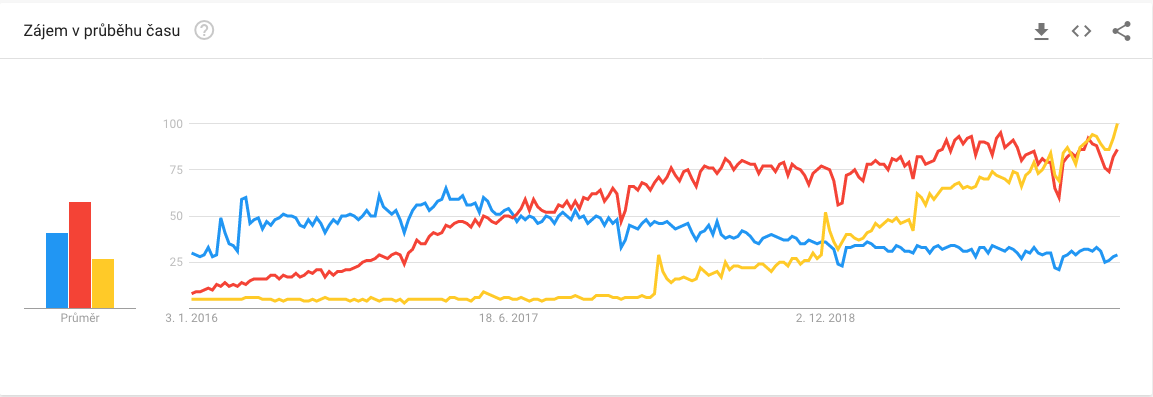
\includegraphics[width=\linewidth]{img/google_trends.png}
	\caption{Srovnání trendů v období 1. 1. 2016 až 11. 4. 2020; červená křivka -- React Native, modrá křivka -- Xamarin, žlutá křivka -- Flutter; -- Zdroj: Google Trends}
	\label{fig:gtrends}
\end{figure}

\subsection{Hodnocení React Native}

%https://github.com/facebook/react-native
% http://pypl.github.io/PYPL.html
React Native je framework pro vytváření nativních mobilních aplikací s JS frameworkem React. React Native je uveden v další kapitole. Tento framework byl vybrán k posouzení především kvůli obrovské komunitě a prověřenosti. Nespornou výhodou frameworku využití jazyku JavaScript, který je třetím nejvíce vyhledávaným programovacím jazykem. JavaScript (resp. EcmaScript) je uveden v následujících kapitolách a nebudou zde jeho výhody rozvedeny. Pod pojmem React Native je zde brána v potaz nadstavba Expo, která dále abstrahuje od nativního kódu.

\begin{table}[h]
	\begin{tabular}{lll}
		Kritérium                       & Hodnocení & Poznámka \\
		Podpora platforem  & 2  & plně podporuje obě mobilní platformy, ale některá API jsou dostupná pouze pro jednu \\
		Rychlost vývoje                 & 1 & kombinace jednoduchého jazyka, dobrých nástrojů a dostupných knihoven \\
		Velikost komunity a dokumentace & 1  & z obrázku  \ref{fig:gtrends}  vyplývá obrovská popularita frameworku v posledních 3 letech \\
		Programovací jazyk              & 1 &          \\
		Vytváření UI                    & 2 &          \\
		Hotové komponenty               & 1 & 24299 balíčků \footnote{\href{https://www.npmjs.com/search?q=react\%20native} k 11. 4.}   
	\end{tabular}
	\caption{Hodnocení React Native}
\end{table}

\subsection{Hodnocení Xamarin}

% https://dotnet.microsoft.com/apps/xamarin

Xamarin je rozšíření platformy .NET pro vývoj multiplatformních aplikací nejen pro mobilní zařízení. Xamarin je postavený nad návrhovým vzorem Model-View-ViewModel, který odděluje uživatelské rozhraní, data a aplikační logiku do separátních vrstev. Uživatelské rozhraní je možno vytvářet deklarativně v jazyku XAML, případně v přímo v jazyku C\#. Změny v uživatelském rozhraní se zajišťují pomocí tzv. data bindingu, tedy navázání proměnné v uživatelském rozhraní s proměnnou ve view modelu. Za Xamarinem stojí technologický gigant Microsoft a je z vybraných technologií nejstarší.

\begin{table}[h]
	\begin{tabular}{lll}
		Kritérium                       & Hodnocení & Poznámka \\
		Podpora platforem & 2 &          \\
		Rychlost vývoje                 & 3 &          \\
		Velikost komunity a dokumentace & 3 &          \\
		Programovací jazyk              & 2 &          \\
		Vytváření UI                    & 2 &          \\
		Hotové komponenty               & 4 & 
	\end{tabular}
	\caption{Hodnocení Xamarin}
\end{table}

\subsection{Hodnocení Flutter}

%https://github.com/flutter/flutter

Flutter je SDK od společnosti Google sloužící pro vytváření "nádherných, rychlých zážitků pro mobil, web a desktop s jedním zdrojovým kódem". Flutter je z vybraných technologií nejnovější, ale výrazně nejrychleji roste. Za obrovskou výhodu Flutteru se dá považovat vývojové prostředí s funkcemi live-reload, které na rozdíl od vývojových prostředí pro Xamarin a React Native má výrazně lepší zapamatování stavu. Flutter byl přímo navržen pro aplikace tohoto typu a obsahuje tedy mnoho optimalizací. Flutter aplikace jsou taktéž výrazně menší na stáhnutí, než aplikace React Native nebo Xamarin. Za nevýhodu Flutteru se dá považovat pouze jazyk Dart, který na rozdíl od C\# nebo JS není stále dostatečně viditelný ve vývojářské komunitě. Podstatnou nevýhodou je nízký počet komponent, vývojáři si tedy musí značnou část komponent psát sami.

\begin{table}[h]
	\begin{tabular}{lll}
		Kritérium                       & Hodnocení & Poznámka \\
		Podpora platforem               & 1 &          \\
		Rychlost vývoje                 & 1 &          \\
		Velikost komunity a dokumentace & 3 &          \\
		Programovací jazyk              & 4 &          \\
		Vytváření UI                    & 1 &          \\
		Hotové komponenty               & 3 & 8450 balíčků \footnote{https://pub.dev/flutter/ k 11. 4.}      
	\end{tabular}
	\caption{Hodnocení Flutter}
\end{table}

\textbf{Výhody}

\begin{itemize}
	\item dynamická technologie,
	\item vysoce kvalitní vývojářské nástroje,
	\item vývíjeno stejnou společností, která stojí za OS Android,
	\item vysoká míra optimalizace,
	\item možnost vytvářet i webové aplikace.
\end{itemize}

\textbf{Nevýhody}

\begin{itemize}
	\item relativně obskurní jazyk Dart,
	\item nížký počet aktuálních návodů,
	\item nížký počet relevantních komponent,
	\item obtížnější zprovoznění + velikost SDK,
	\item komunita nemá stále stejnou velikost jak komunita React a React Native.
\end{itemize}

\subsection{Vybraná technologie}

Pro řešení práce byla vybraná technologie React Native (resp. Expo), jelikož ze srování vyšla nejlépe. Dále bylo rozhodnuto o využití nadstavby TypeScript na JS a správce stavů MobX. Popis technologie je uveden v další kapitole.

\section{React Native}

Technologie React Native je postavena na mnoha dílčích částech, které se musí uvést pro komplexní pochopení React Native samotného.

\subsection{JavaScript a EcmaScript}

% https://www.computerworld.com/article/3458282/the-a-z-of-programming-languages-javascript.html
% https://web.archive.org/web/20150910072359/http://adaptivepath.org/ideas/ajax-new-approach-web-applications/
% https://github.com/nodejs/node-v0.x-archive/tags?after=v0.0.4
% https://github.com/angular/angular.js/releases?after=v0.9.4

JavaScript je multiparadigmatický interpretovaný slabě typovaný programovací jazyk určen primárně pro webové prohlížeče. JavaScript vznikl v roce 1995 Brendanem Eichem pod firmou Netscape. Cílem bylo přidat interaktivitu do čistě statických webových stránek a reagovat tedy na interakci uživatele i jinak, než jen přenačtením celé stránky. S obrovským rozvojem domacích počítačů přišel i rozvoj internetu a internetových prohlížečů. Od již zmíněného roku 1995 do roku 2004 byl trh webových prohlížečů dominován verzemi prohlížeče Internet Explorer od firmy Microsoft, která přišla s vlastní implementací JavaScriptu, tzv. JScriptem. Kvůli nespolupráci mezi vývojáři různých implementací vznikaly v jazyku nekonzistence mezi prohlížeči, ale i přesto se jazyk určitým směrem ubíral. V roce 2005 byl zaveden termín AJAX, který znamenal obrovskou změnu v interaktivitě webových aplikací. Zkratka AJAX, neboli Asynchronous JavaScript and XML byla revoluční ve změně komunikace serveru s JavaScriptem. JavaScript dříve obdržoval fragmenty HTML od serveru a tím aktualizoval stránku, případně se stránka po každé významné interakci uživatele překreslila sama. AJAX zavedl možnost jak na pozadí získat z určitých vstupů určité výstupy v lépe strojově zpracovatelném formátu. S tímto revolučním nápadem začaly vznikat první JavaScript knihovny a frameworky pro interaktivní webové \emph{aplikace}, např. dodnes používaná knihovna jQuery. Dalším podstaným krokem byl vývoj webového prohlížeče Google Chrome, resp. jeho JavaScript interpreteru V8. V8 je open-source JS interpreter s just-in-time kompilací, který byl revoluční primárně ve své rychlosti. Tento interpreter byl také zařazený i do aplikací mimo webové prohlížeče, čímž se případy užití pro jazyk výrazně rozšířily. Zde za zmínku stojí node.js (vznik datovaný do roku 2009) a jeho ekosystém NPM, který je rozveden níže. Dalším milníkem podstatným pro tuto práci je rozšíření frameworků pro single-page aplikace, které emulují chování běžných nativních aplikací v prohlížeči. Aplikace fungují na komponentovém systému a aktualizují se při změně dat. Aplikace jsou tedy uživatelsky i programátorsky komfortnější a jejich vývoj je značně rychlejší. Aplikace tohoto typu se rozšiřují od roku 2010.

%https://tc39.es/ecma262/#sec-overview

EcmaScript je specifikací jazyka JavaScript, kterou musí každé prostředí implementovat. EcmaScript definuje pouze jazyk, ale ne objekty kontextu, např. ve webových prohlížečích není definována interakce s DOM. JavaScript je ale dnes používán i na serverech, embedded zařízeních či jako skriptovací jazyk mnoha programů, bylo nutno od těchto specifikací abstrahovat, aby základ jazyka zůstal stejný. Tímto ale vznikají jisté nekonzistence mezi implementacemi v různých prohlížečích, obzvláště napříč verzemi, kde se jádro interpreteru již neaktualizuje. Pro řešení těchto problémů byly mimojiné zavedeny tzv. \emph{polyfilly}, které doplňují určité funkce z nové verze zpětně do staré a \emph{transpilátory} (např. Babel), které některé nové jazykové funkce umí převést do verze ES kompatibilní se starým interpreterem. V čase psaní této práce je aktuální verzí EcmaScript 2018.

S příchodem node.js ekosystému vznikl v JS světě koncept NPM balíčků. Balíčky jsou publikovány autorem do centrálního repozitáře balíčků a každý programátor si tento balíček může nainstalovat. Balíčky jsou typicky knihovny, malého či velké rázu, frameworky, nástroje, samostatné programy či kompletní projekty. Koncept balíčků výrazně urychluje vytváření projektů a instalaci knihoven. Příklady práce s NPM jsou uvedeny v kapitolách React a React Native.

\subsection{TypeScript}

TypeScript je nadstavbou jazyka ECMAScript. TypeScript rozšiřuje jazyk o kontrolu typů a běžné konstrukty známé z jiných jazyků (např. rozhraní). Jazyk je plně kompabitilní s ES, ale samotný TypeScript není přímo většinou interpeterů spustitelný. Při sestavování projektů s TypeScriptem se využívá tzv. transpilace, převedení z jednoho programovacího jazyka do druhého. TypeScript vyšel v roce 2012 pod křídly firmy Microsoft a je aktivně vyvíjen dodnes.

TypeScript se běžně využívá ve větších projektech především kvůli prevenci chyb a zvýšení přehlednosti kódu. Vývojová prostředí taktéž lépe rozumí typovaným jazykům a tímto se může i zrychlit vývoj. Zaintegrovat TypeScript do existujícího projektu také není problém, jelikož jakýkoliv validní kód v ES je validní kód v TypeScript.

\subsection{React}

\begin{figure}
	\begin{center}
		
\includegraphics[width=70mm]{img/react-logo.png}
	\end{center}
	\caption{Logo React -- zdroj: Facebook Inc.}
\end{figure}

% https://reactjs.org/

React je JS knihovna pro vytváření uživatelských rozhraní (ref) od společnosti Facebook. React je deklarativní, component-based knihovna s velkým spektrem potenciálních využití. Jako jiné moderní UI knihovny v JS je taktéž reaktivní, při změně dat se překreslí uživatelské rozhraní pouze tam, kde musí. Deklarativnost Reactu spočívá právě v zakládání si na komponentách. Uživatelské rozhraní se skládá z předdefinovaných, uživatelem vytvořených nebo komunitou vytvořených komponentách, které se do sebe skládají. Každá komponenta si uchovává vlastní data (popř. stav v atributu props) a může komunikovat s nadřazenou či podřazenou komponentou pomocí událostí nebo předáváním dat. Komponenty jsou v Reactu definovány pomocí speciální kombinace JS a HTML, tzv. JSX. JSX je vždy obaleno elementem, který může být HTML elementem či jinou komponentou. V JSX se na rozdíl od běžného HTML může vyskytovat aplikační logika, uvozena v složených závorkách.  Níže je uvedena kompletní komponenta z oficiální dokumentace (ref!), která při využití této komponenty \verb|<HelloComponent name="world"/>| vypíše do div tagu Hello world.

\begin{lstlisting}[language=JavaScript, caption=React komponenta]

class HelloMessage extends React.Component {
	render() {
		return (
			<div>
			Hello {this.props.name}
			</div>
		);
	}
}
\end{lstlisting}

Případně pro ilustraci podmíněné logiky lze uvést následující příklad:

\begin{lstlisting}[language=JavaScript, caption=React komponenta s podmínkou]

class ConditionalComponent extends React.Component {
	render() {
		return (
			<div>
				{this.props.sayHello?
					<span>
							Hello {this.props.name}
					</span>
					:<span>
							Goodbye {this.props.name}
					</span>
				}
			</div>
		);
	}
}
\end{lstlisting}

Příklad využívá slabého typování JS, stačí tedy pouze aby sayHello bylo pravdivé (případně \emph{truthy} -- aby se alespoň evaluovalo na pravdu) a provede se správná část JSX. Podmínka je zde zapsána ve formě ternárního operátoru, klasická if struktura by musela být ve vlastní funkci.

Komponenty mohou samozřejmě být výrazně komplexnější, např. mohou obsahovat funkce vracející JSX a tím být výrazně přehlednější. Mimo JSX mohou obsahovat metody a atributy pro práci s daty, např. pro získání dat ze serveru nebo k vyfiltrování dat. Tyto funkce mutují stav komponenty pomocí funkce  \verb|setState|, která mění stav komponenty ( \verb|this.props.*| v ukázce) a zároveň zajistí její překreslení, pokud je to nutné. Změna jména by tedy mohla být docílena i zavoláním \verb|this.setSate({name: 'svete'});| z metody v komponentě.

React aplikce se ale nemusí skládat jen z komponent, modulární systém nového JS umožňuje jednoduše zakomponovat do aplikace i kód mimo komponenty. Komponenty ale stále zůstanou centrálním bodem aplikace a je tedy výhodné aplikaci strukturovat do většího počtu malých komponent kvůli přehlednosti, testovatelnosti a znovupoužitelnosti.

\subsection{React Native}

React Native je framework pro vytváření mobilních aplikací postavený nad knihovnou React, opět od společnosti Facebook. React Native, na rozdíl např. od progresivních webových aplikací se chová jako nativní aplikace -- aplikace je vykreslovaná nativním kódem a nemá omezení typická pro webové aplikace, např. v přístupu k určitým API. Rozdílem od čistého Reactu je omezený výběr komponent a výrazně odlišný způsob jejich stylování. Zatímco v React je možno využít plného rozsahu CSS a všech HTML elementů, v React Native jsou v základu poskytnuty jen určité komponenty, nejpodstnější z nich jsou View, Text a Image. View je kontejnerovým prvkem, který nemá žádné specifikované využití. Používá se často pro držení jiných komponentů či stylování. Text je jediná komponenta, která může obsahovat text. Image je komponenta obsahující obrázek z lokálního nebo vzdáleného zdroje. Jsou poskytnuty i další komponenty pro formulářová pole (TextInput, Button, Picker), indikátory aktivity a seznamy. Jiné komponenty se dají složit z těchto základních komponent, jejich událostí a jejich stylů. 

% co sem dál napsat?

React Native umožňuje psát nativní kód a mnoho komponent této skutečnosti využívá. Nevýhodou tohoto přístupu je, že nativní kód se musí psát v Javě pro Android a v jazyce Swift pro iOS. Tímto vzniká prakticky vzato duplicita kódu a dvojnásobná nutnost testovat.

\subsection{MobX}

% https://books.google.nl/books?id=ALFmDwAAQBAJ&pg=PP1&lpg=PP1&dq=michel+weststrate+mobx+quick+start+guide:+supercharge+the+client+state+in+your+react+apps+with+mobx&source=bl&ots=D460fxti0F&sig=ivDGTxsPNwlOjLHrpKF1nweZFl8&hl=nl&sa=X&ved=2ahUKEwiwl8XO--ncAhWPmbQKHWOYBqIQ6AEwAnoECAkQAQ#v=onepage&q=michel%20weststrate%20mobx%20quick%20start%20guide%3A%20supercharge%20the%20client%20state%20in%20your%20react%20apps%20with%20mobx&f=false

% str. 12

MobX je knihovna pro reaktivní správu stavu aplikace (ref)
. Knihovna zavádí koncept pozorovatelného stavu, tedy že se na objekt či kolekci objektů naváže pozorovatel, který automaticky zajišťuje změnu stavu pro React při změně pozorovaného. Tímto se výrazně zjednodušuje vývoj React Native aplikací tím, že se pro každou změnu stavu nemusí volat setState a nemusí se využívat pouze proměnné props. Na rozdíl od častěji využívané knihovny Redux je knihovna výrazně úspornější, přičemž obě knihovny zajišťují, že data tečou ze zdroje k cíli pouze jedním směrem a že na správné změny komponenty reagují.

\subsection{Expo}

% https://docs.expo.io/versions/latest/
% https://flatlogic.com/blog/why-i-don-t-want-to-use-react-native-with-expo/

Expo je součástí nástrojů a služeb postavených nad React Native a nativními platformami sloužící k vývoji, sestavení, nasazení a rychlé iteraci iOS, Android a webových aplikací s jednotným zdrojovým kódem (ref). Expo je abstrakce oddělující React Native kompletně od nativního kódu a tedy od nutnosti vyvíjet ve třech jazycích. Expo poskytuje většinu API pro běžné mobilní aplikace (podstatnou výjimkou je Bluetooth a nákupy v aplikaci), nástroje pro rapidní vývoj a cloudovou infrastrukturu pro sestavení, není tedy nutné pro sestavení např. iOS aplikace vlastnit stroj s operačním systémem MacOS. Nástroje pro rapidní vývoj jsou obrovské plus platformy Expo -- JS se sestaví na stroji vývojáře, odešle se na servery Expo a je možné projekt spustit na jakémkoliv zařízení za pomocí speciální mobilní aplikace a QR kódu. Z tohoto zařízení je v realném čase možné sledovat běh událostí a ladících zpráv. 

Mezi nevýhody Expo se udává následující:

\begin{itemize}
	\item nepodporuje všechny API,
	\item nejsou podporované všechny způsoby běhu na pozadí,
	\item aplikace jsou výrazně větší (min. 25 MB),
	\item push notifikace jsou možné pouze přes infrastrukturu Expo,
	\item minimální podporovaná verze je Android 5 a iOS 10,
	\item zdlouhavé čekaní na sestavení ve veřejné infrastruktuře.
\end{itemize}

Mezi chyby se uvádí i nemožnost využívat nativní knihovny, ale zde těžko posoudit, zda se jedná o výhodu nebo nevýhodu. Expo slibuje některé z těchto problémů vyřešit, ale jedná se o dlouhodobé problémy a žádné odhadované datum řešení není stanoveno. 

Při vývoji čistě React Native aplikací a Expo aplikací není poznat téměř žádný rozdíl, jediný rozdíl je v použitých knihovnách -- knihovny nesmí využívat nativní kód a pro práci s systémovými API se využívá API poskytované balíčkami Expo.

Pro vytvoření Expo aplikace stačí zadat následující kód do příkazové řádky:

\begin{lstlisting}[language=Bash, caption=Vytvoření základní struktury aplikace]
npm install --global expo-cli
expo init mobilni-aplikace
\end{lstlisting}

Expo automaticky vytvoří doporučovanou adresářovou strukturu a ukázkové komponenty. Většina projektů má tedy stejný základ a vývojáři by se v nich měli lépe vyznat. Pro spuštění sestavovacích nástrojů a live-reload funkce stačí do příkazové řádky zadat:

\begin{lstlisting}[language=Bash, caption=Spuštění mobilní aplikace na virtuálním stroji nebo připojeném zařízení]
expo start --android #platforma Android
expo start --ios #platforma iOS
\end{lstlisting}

Po spuštění příkazu se načte ve webovém prohlížeči obrazovka obsahující log sestavovacího nástroje (Metro Bundler), ladící výstupy aplikace, seznam proveditelných akcí a QR kód pro spuštění aplikace na jakémkoliv mobilním zařízení s klientskou aplikací Expo. Z této obrazovky je taktéž možné projekt publikovat přes cloudové nástroje Expo. Alternativní způsob je popsán v následující kapitole.

\begin{figure}[h]
	\begin{center}
		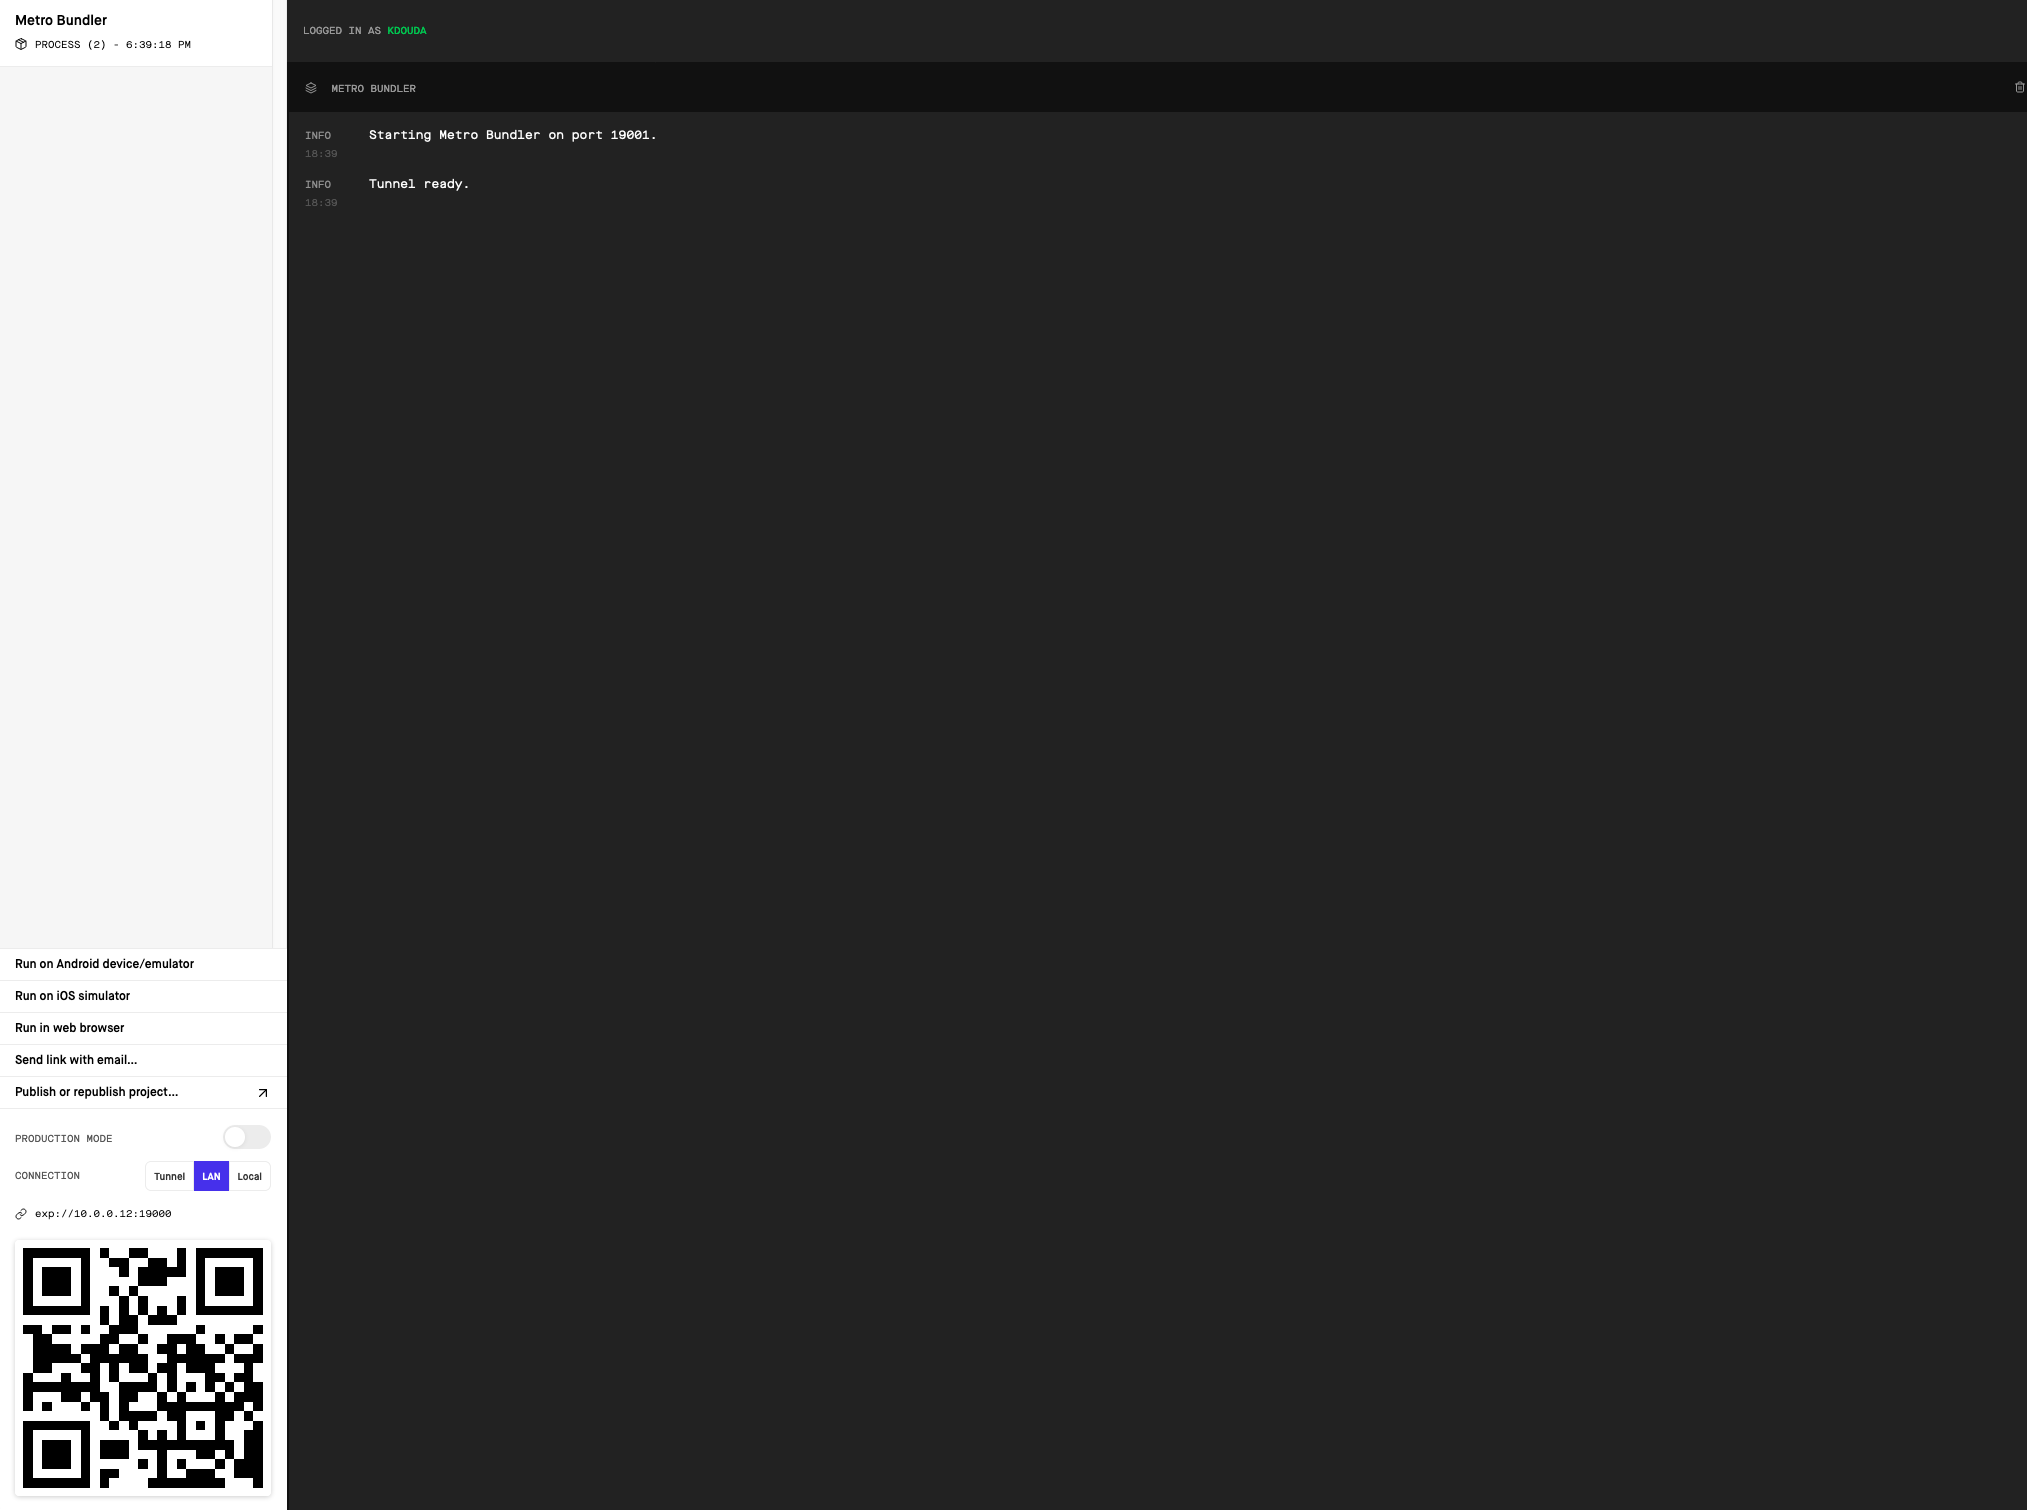
\includegraphics[width=140mm]{img/expo.png}
	\end{center}
	\caption{Expo -- zdroj: autor}
\end{figure}

\subsection{TurtleCLI}

TurtleCLI je nástroj pro sestavení Expo aplikací z příkazové řádky. Nástroj je určen pro uživatele, kteří si nepřejí využívat infrastruktury poskytované od Expo pro sestavování vlastních aplikací, ale přejí si aplikaci sestavit například na vlastním stroji nebo na vlastním nástroji kontinuální integrace. Autor práce vybral tuto technologi z důvodu vysoké vytíženosti veřejné infrastruktury společnosti Expo (varianta nazývaná Community), kde jeho build ve frontě čekal v jednotkách hodin, než se dostal na řadu. Společnost Expo nabízí placenou variantu svých služeb, ve kterých avizuje výrazně vyšší rychlost odbavení, než u varianty zdarma a nástroje pro týmovou práci. Za značnou nevýhodu se taktéž může brát fakt, že kód je vždy odesílán třetí straně k sestavení, což pro mnoho firem může být nepřípustné. Oproti tomu provozování na vlastní infrastruktuře skýtá mnoho potenciálních výhod, za zmínku stojí napojení na firemní CI procesy, testovací infrastrukturu, rapidní nasazení mnoha paralelních větví do testovacích kanálů, jednodušší napojení sestavení na jiné akce. Níže je uvedena tabulka popisující podstatné rozdíly mezi jednotlivými způsoby sestavení Expo aplikací. 

\begin{table}[h]
	\begin{tabular}{llll}
		Kategorie                        & Community         & Priority      & Vlastní infrastruktura                 \\
		Cena                             & zdarma            & 29 USD / měs. & cena výpočetního výkonu                \\
		Čekací doba na začátek sestavení & cca. 1h           & minuty        & ihned                                  \\
		Složitost zprovoznění            & součástí expo-cli & triviální     & dle zvolené varianty, nepříliš náročné \\
		Provázanost s Expo               & vždy              & vždy          & dle zvolené varianty                  
	\end{tabular}
\end{table}